\section{Experiments}
\label{sec:experiments}

\begin{figure}[t]
\centering
	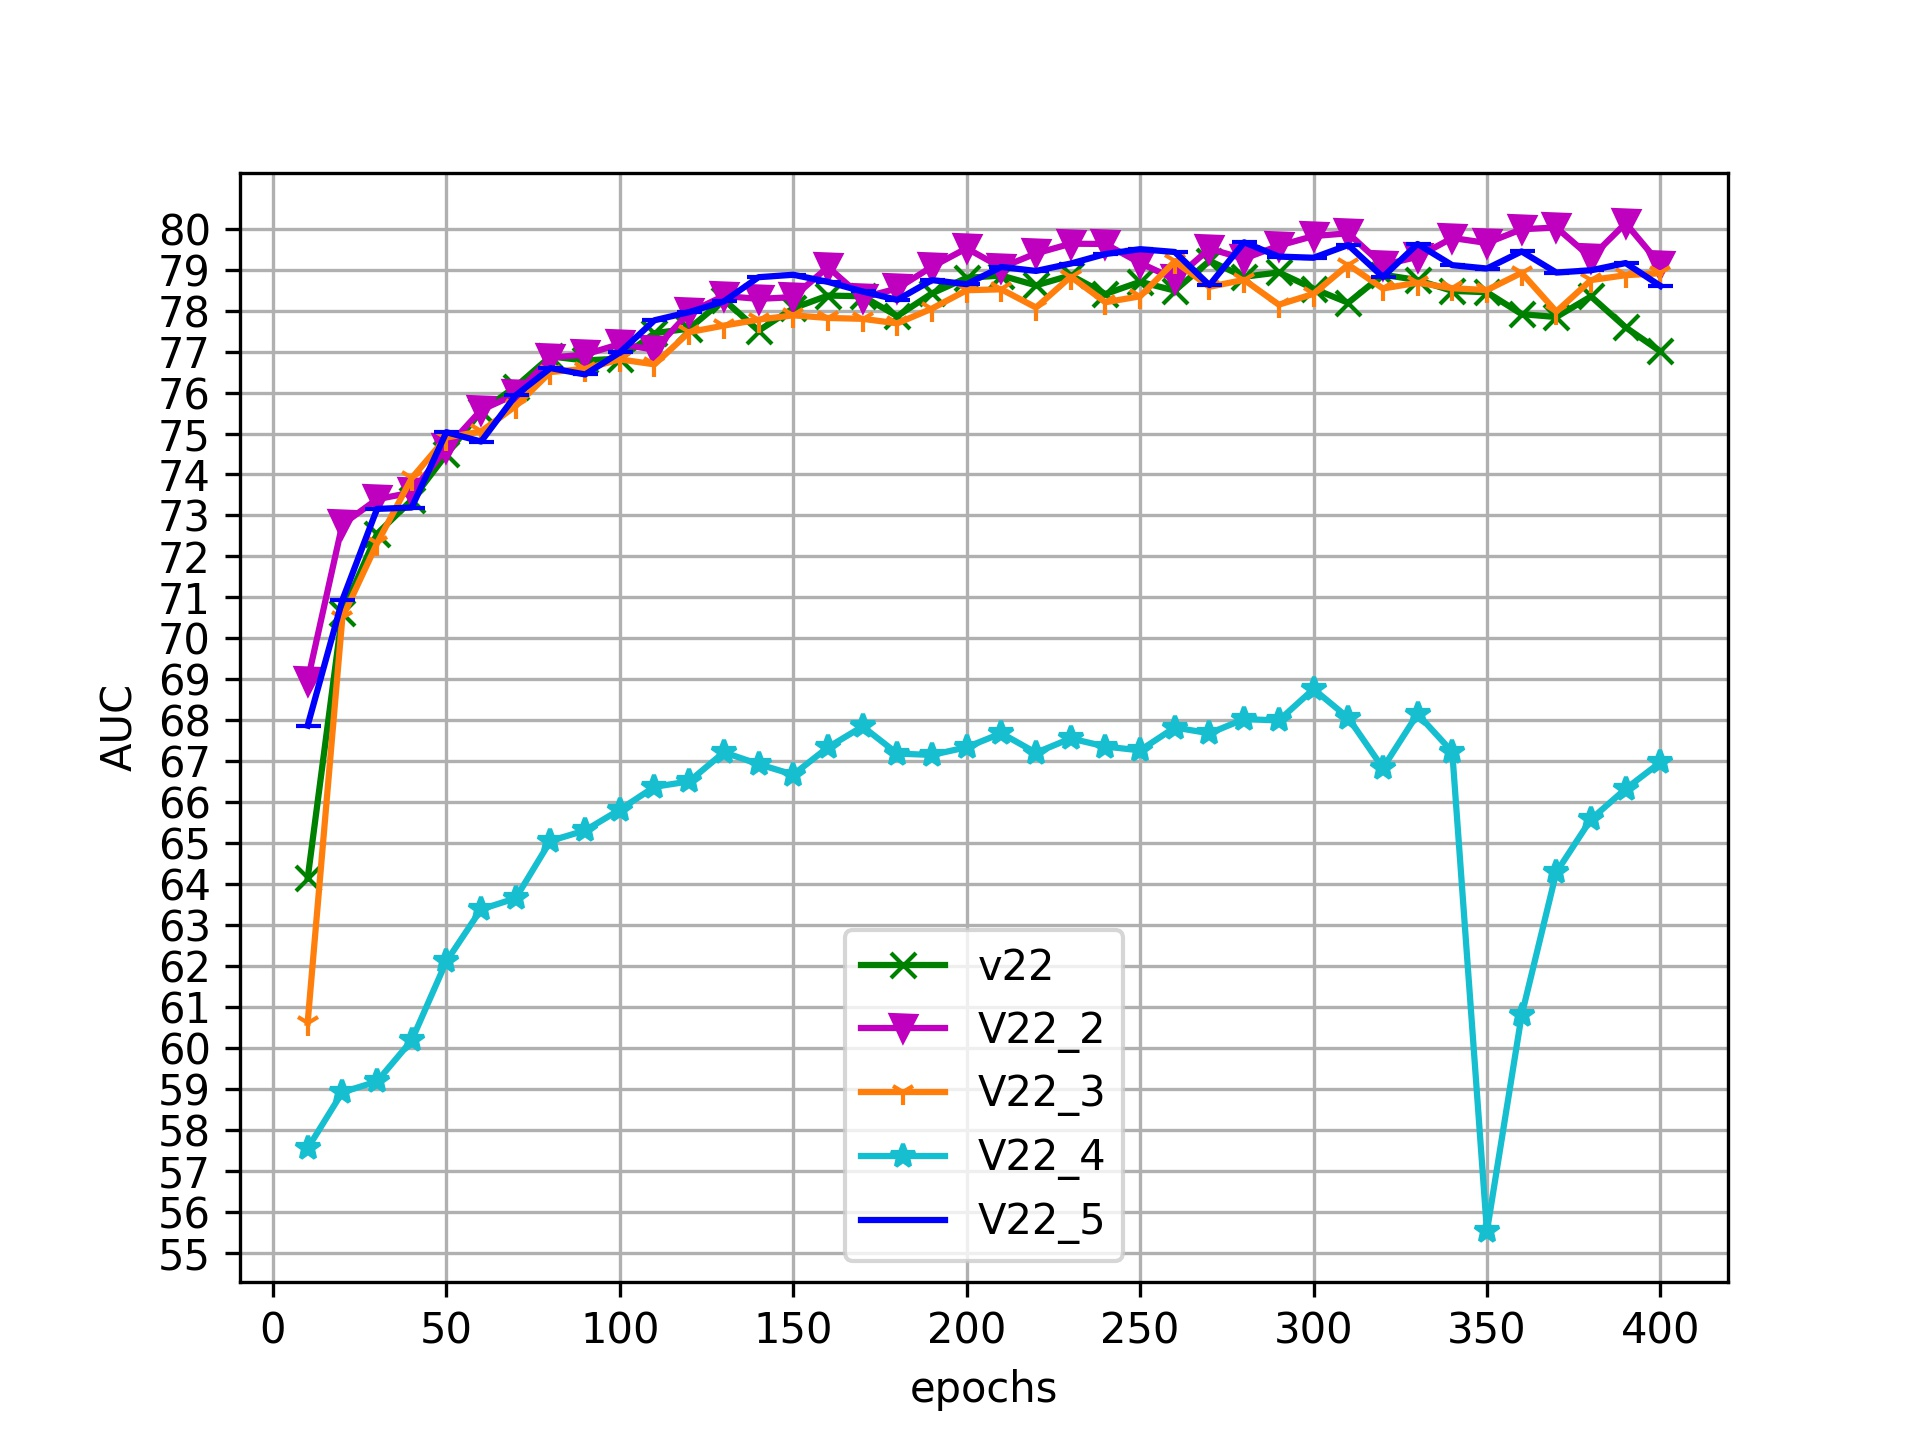
\includegraphics[trim=0 0 0 0, clip, width=1.\linewidth]{images/exp_1.jpg}
	\caption{Performance comparison changing the number of frames (from 1 to 5) in input of the Short-term memory module. NF: number of frames. \mnote{memento risolvere il crollo di NF1}}
	\label{fig:num-frames-vst}
\end{figure}

\begin{figure}[t]
\centering
	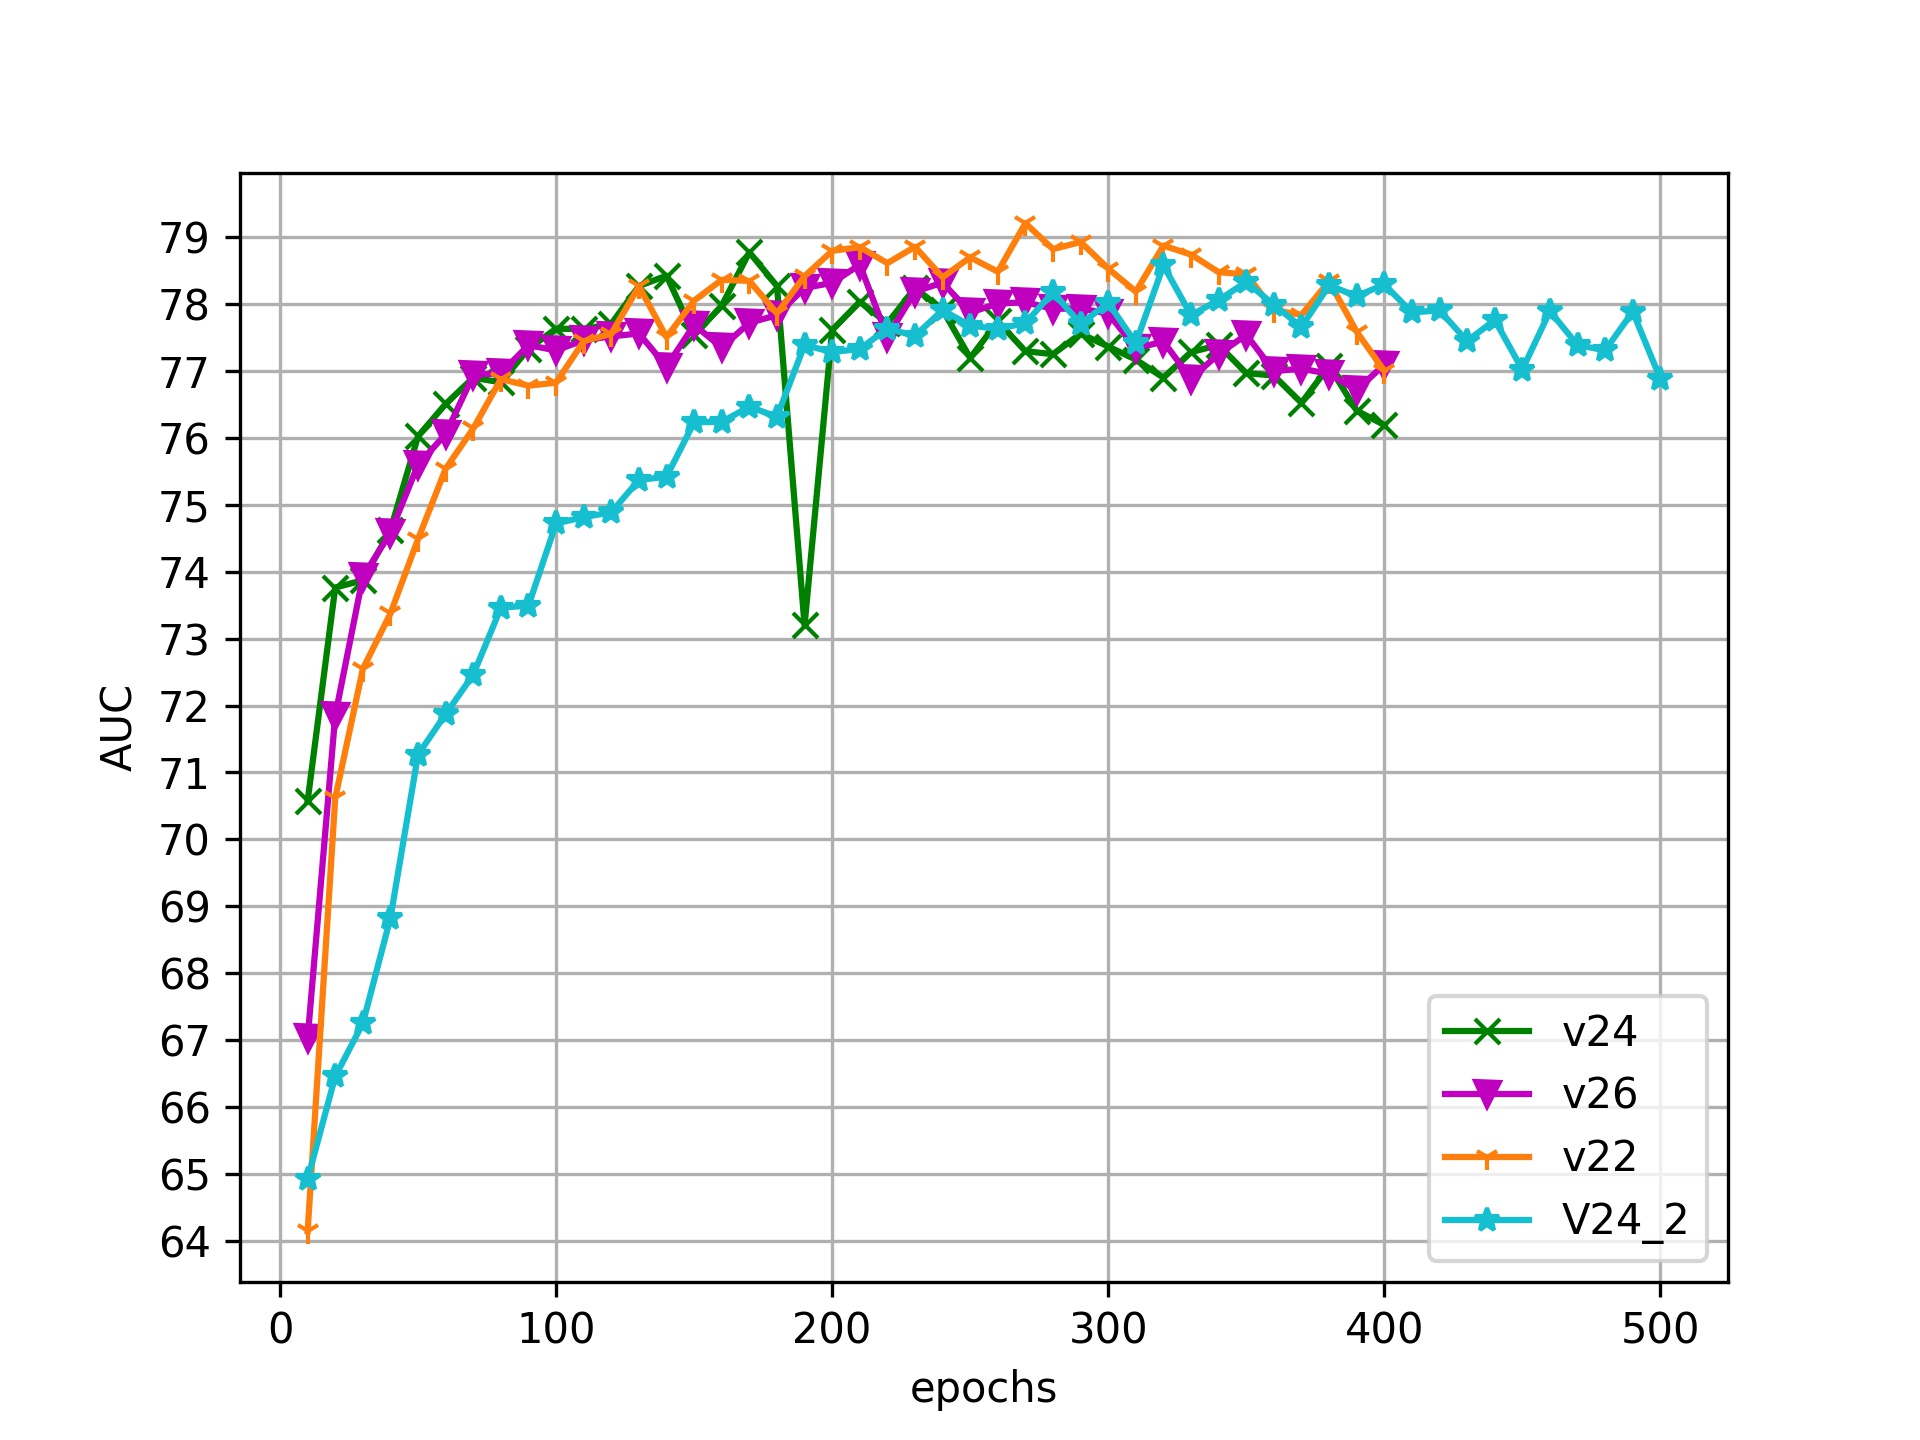
\includegraphics[trim=0 0 0 0, clip, width=1.\linewidth]{images/exp_2.jpg}
    % TODO aggiorna caption!
	\caption{Performance comparison changing the number of LSTM cells (from 0 to 4) that form the long-term memory. "LSTM 2 cells" is NF 3 of previous experiment in Fig.~\ref{fig:num-frames-vst}.}
	\label{fig:num-memory-cells}
\end{figure}

\begin{figure}[t]
\centering
	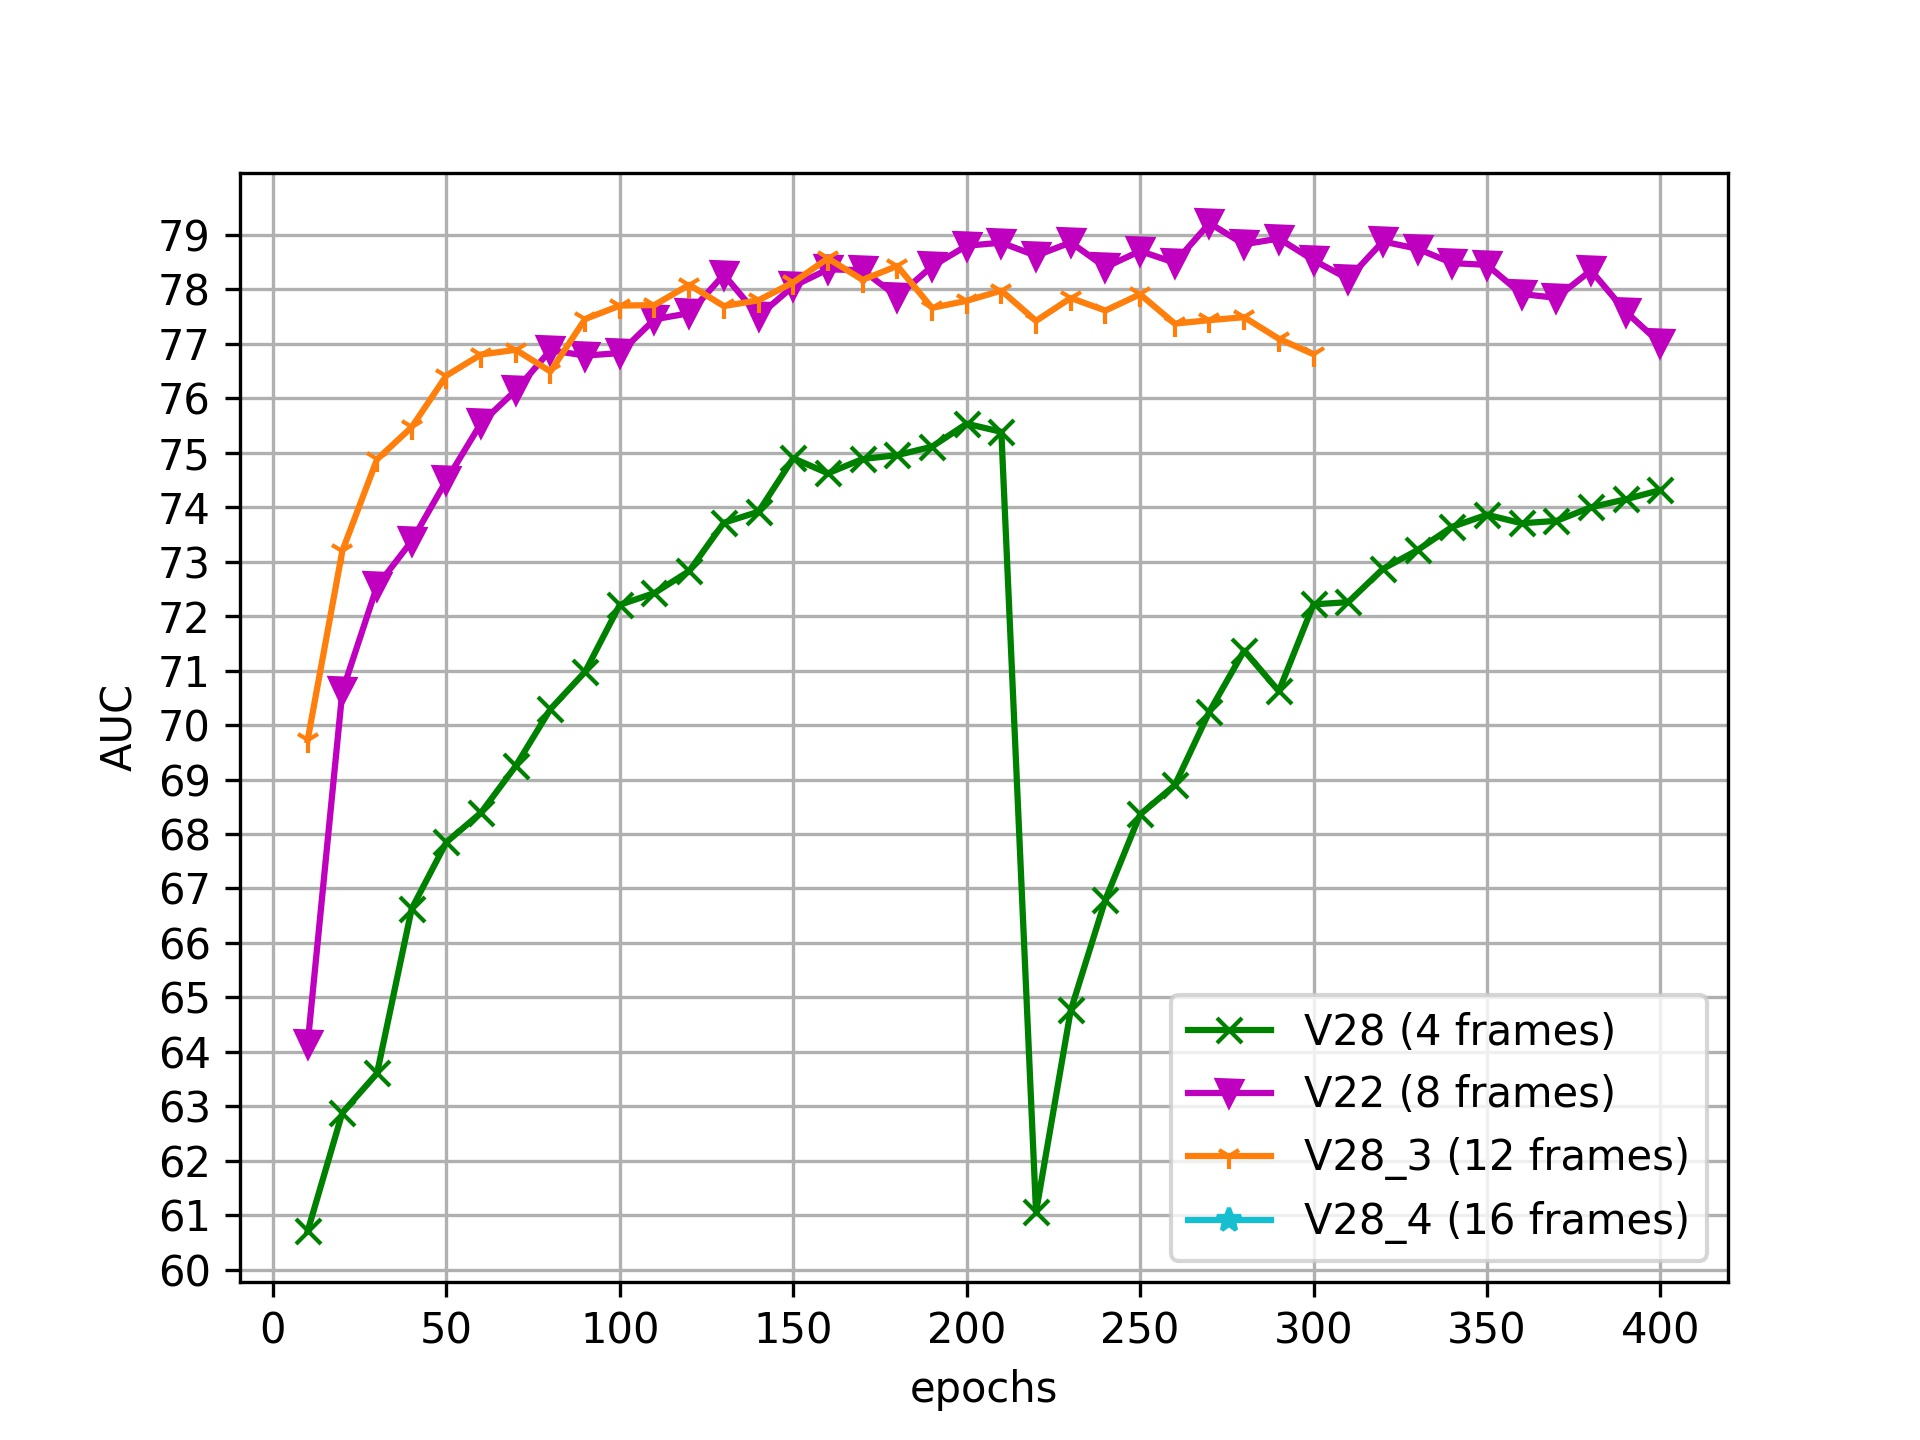
\includegraphics[trim=0 0 0 0, clip, width=1.\linewidth]{images/exp_3.jpg}
    % TODO aggiorna caption!
	\caption{Performance comparison changing the video clip length (from 4 to 16). The "8 frames" configuration is the NF 3 configuration of previous experiment in Fig.~\ref{fig:num-frames-vst}. \lnote{fix labels}}
	\label{fig:random-batch}
\end{figure}

\begin{table}[b]
	\footnotesize
	%\setlength{\tabcolsep}{1.2pt}
	\begin{center}
		\begin{tabular}{!r|^l|^l|^c|}
			\# & Method & Input & $AUC$ \\
			\hline\hline
	   	              1 & ConvAE \cite{hasan2016learning} & Gray & 64.3 \\
			        2 & ConvAE \cite{hasan2016learning} & Flow & 66.3 \\
                    3 & ConvLSTMAE \cite{chong2017abnormal} & Gray & 53.8 \\
                    4 & ConvLSTMAE \cite{chong2017abnormal} & Flow & 62.5 \\
                    5 & AnoPred \cite{liu2018future} & RGB & 67.5 \\
                    6 & AnoPred \cite{liu2018future} & Masked RGB & 64.8 \\
            \hline
                    7 & FOL-Ensemble \cite{9712446} & RGB + Box + Flow + Ego & 73.0 \\
                    8 & STFE \cite{zhou2022spatio} & RGB + Flow & 79.3 \\
            \hline
                    9 & Our (MOVAD) & RGB (320x240) &   \\
                    10 & Our (MOVAD) & RGB (640x480) &   \\
\end{tabular}
	\end{center}
	\caption{Benchmarks of VAD (Video Anomaly Detection) methods on the DoTA dataset.}
	\label{tab:sota-vad-auc}
\end{table}

% TODO visualizza anche la colonna OO e VO? (VO and OO columns are not shown because they do not contain anomalous traffic participants)
\begin{table*}[ht]
	\footnotesize
	\setlength{\tabcolsep}{5.0pt}
	\begin{center}
		\begin{tabular}{!l|^c|^c|^c|^c|^c|^c|^c|^c|^c|^c|^c|^c|^c|^c|}
			Model & $ST$ & $AH$ & $LA$ & $OC$ & $TC$ & $VP$ & $ST*$ & $AH*$ & $LA*$ & $OC*$ & $TC*$ & $VP*$ & $VO*$ & $OO*$ \\
			\hline\hline
                AnoPred \cite{liu2018future}        & 69.9 & 73.6 & 75.2 & 69.7 & 73.5 & 66.3 & 70.9 & 62.6 & 60.1 & 65.6 & 65.4 & 64.9 & 64.2 & 57.8 \\
                AnoPred \cite{liu2018future} + Mask & 66.3 & 72.2 & 64.2 & 65.4 & 65.6 & 66.6 & 72.9 & 63.7 & 60.6 & 66.9 & 65.7 & 64.0 & 58.8 & 59.9 \\
                FOL-STD \cite{9712446}              & 67.3 & 77.4 & 71.1 & 68.6 & 69.2 & 65.1 & 75.1 & 66.2 & 66.8 & 74.1 & 72.0 & 69.7 & 63.8 & 69.2 \\
                FOL-Ensemble \cite{9712446}         & 73.3 & 81.2 & 74.0 & 73.4 & 75.1 & 70.1 & 77.5 & 69.8 & 68.1 & 76.7 & 73.9 & 71.2 & 65.2 & 69.6 \\
                % STFE gli manca la colonna VP*!
                % STFE ha dei risultati non molto chiari.
                STFE \cite{zhou2022spatio} & 75.2 & 84.5 & 72.1 & 77.3 & 72.8 & 71.9 & 80.6 & 65.6 & 69.9 & 76.5 & 74.2 & N.D. & 75.6 & 70.5 \\
                Our (MOVAD) &      &      &      &      &       &      &      &      &      &      &      &      &    &   \\
                  % 
                  v30 & 84.2 & 85.8 & 83.6 & 82.3 & 84.9 & 83.2 & 73.7 & 71.6 & 73.0 & 80.6 & 78.0 & 73.9 & 80.2 & 77.6 \\
\end{tabular}
	\end{center}
	\caption{Detection accuracy for each individual accident category (AUC) on VAD task. "*" indicates non-ego anomaly categories. \lnote{mettiamo tutte le classi?}\vnote{secondo me si, sarebbe scorretto altrimenti, piuttosto evidenziamo le buone prestazioni in video ego}} 
	\label{tab:sota-vad-auc-per-class}
\end{table*}

\noindent\textbf{Dataset}.
We perform our tests on the DoTa dataset \cite{9712446}.
It contains 4677 videos taken from YouTube channels, with a resolution of $1280 \times 720$, annotated with information about the start and end of the anomaly, the category (10 in total) and the bounding boxes of the objects or persons involved.
The videos were recorded in different countries and with different light and weather conditions.
The dataset is split in approximately $70\%$ training and $30\%$ validation.
Our benchmarks are related to the Task~1~\cite{9712446}, the (frame-level) Video Anomaly Detection.
Our training and evaluation takes place in the most realistic, and most interesting condition from our point of view, online scenario.
That is, in which the model does not know what will happen in the future, but only know the present and the past.

\noindent\textbf{Evaluation Metrics}.
To evaluate the performance of the models, we use the well-known Area Under Curve (AUC) metric at frame-level.
This metric evaluate how well the model temporally locate the anomaly in the videos. 

\noindent\textbf{Implementation details.}
The results of the models with which we compare our model, are taken from the respective papers.
We perform the training on a single machine with 1 A100 GPU.
We use the Stochastic Gradient Descent (SGD) optimization algorithm with a learning rate of 0.0001, a momentum of 0.9, video clip length 8 and batch size 8.
We use SGD instead of Adam because in our experiments the latter led the training too much unstable, leading the model to diverge after a few epochs.

\noindent\textbf{Training details.}
Because the videos contain a non-uniform number of frames, to be able to fast training with batch-size major than one, we fixed the number of frames for each video taken into account, that is video clip length.
At each iteration we chose the starting frame for each video, adjusting the ground-truth accordingly, in a way to offer to the network as diverse as possible training and reduce the effect of overfitting.
Unless otherwise specified, the model is initialized using a uniform distribution for Linear weights, with a (semi) orthogonal matrix for LSTM modules and zero for bias parameters, the VST weights are initialized with a model pretrained on Something-Something v2 and input video shape is $320 \times 240$.

\subsection{Ablation study}

% class weight loss
% 2xsoftmax vs 1x
% learning rate differences (sto finendo l’esperimento con multipli lr)

\noindent\textbf{Short-term memory module.}

% v22: numero di frames in input
In this experiment, we empirically show the effects of the input frames to the Short-term memory module, varying the number of frames processed by the VST at each step.
The results are displayed in the Fig.~\ref{fig:num-frames-vst}.
As we expected, taking into account only the current frame is the worst situation, because most of the anomalies can be recognized by processing a wider time frame.
With 4 frames we have the best result.
Increasing the number of frames processed at each step has a much more limited effect.
While, already with 5 frames the effect become counterproductive.

% (no) v23: rand frame order (v17) vs normal
% v29_2, v29, v22: training from scratch vs pretrained (imagenet vs smth2smthv2)

\noindent\textbf{Long-term memory module.}
% posizione dell'lstm senza / prima / dopo / prim + dopo / gru
% v24_4: senza lstm
% v24, v22, v24_2: 1/2/3 # celle lstm
% v26, v26_2, v26_3: 1/2/3 # celle gru
% (no) v27, v27_2: pre + post lstm (1 cell) + saliency (?), pre + post lstm (1 cell)
In this experiment, we evaluate the long-term memory effect on the classification capability.
In Fig.~\ref{fig:num-memory-cells}, we compare the network with and without the LSTM long-term memory.
For the long-term memory, we test the LSTM and the GRU \cite{chung2014empirical} modules, with a number of cells varying from 1 to 4.
To make the Figure easier to read, the GRU results are not shown, but the trend does not differ much from the LSTM module. 
The effect introduced by the memory cells is evident.
Having no cell makes training slower in saturating performance and reach lowest AUC value.
With a cell, the performances saturate very quickly, with a slow degradation during the rest of the epochs.
By increasing the number of cells, the achievement of the maximum peak is slowed down over time, but in absolute value it is higher, converging towards similar values.
The maximum value is reached by 2 LSTM cells around epoch 270.
\lnote{check se aggiungere pezzo relativo a: alla fine la migliore è con 3 celle perchè il picco lo raggiunge verso 400 epoche quando interessa maggiormente a noi}

%\noindent\textbf{Saliency module.}
% v25, v22: con/senza/versione ridotta della saliency
%In this experiment, we evaluate the effect of the saliency branch.

\noindent\textbf{Video clip length.}
% v22, v28: random_batch 4/8/12/16/20/24: describi la modalità di addestramento -> per usare un batch size > 1 si è scelto di selezionare un numero max di frame da elaborare a ogni iterazione. per aggiungere diversità al training, il punto di inizio per ogni video viene scelto in modo casuale a ogni iterazione, adattando di conseguenza il ground-truth
As mentioned in training details subsection, at each iteration and separately for each video, a random starting point is selected and a fixed number of frames is inserted inside the batch to train the network.
In Figure \ref{fig:random-batch}, we evaluate the effect of the size of the video clip length.

\noindent\textbf{MOVAD model}
% input shape
% versione finale vs resto del mondo su dota, and: 
%   - Phantom: https://paperswithcode.com/paper/approaches-toward-physical-and-general-video
%   - ShanghaiTech: https://paperswithcode.com/sota/anomaly-detection-on-shanghaitech
%   - CUHK Avenue: https://paperswithcode.com/sota/anomaly-detection-on-chuk-avenue
%   - UCSD Ped2: https://paperswithcode.com/sota/abnormal-event-detection-in-video-on-ucsd
Finally, in Table \ref{tab:sota-vad-auc} we compare our architecture performance with state of the art models.
Table \ref{tab:sota-vad-auc-per-class} shows results per class.